Three operations may be performed on a RT Container: (a) the RT Container may be \emph{started}; (b) the RT Container may be \emph{stopped}; and (c) the RT Container may be \emph{notified}.

A RT Container may be in two states: STOPPED or STARTED. Initially, by default, the container is in state STOPPED. When a RT Container is started, the behaviour shown in the activity diagram in the left-hand side of figure \ref{fig:RTStartStop} is executed. The Start operation only has an effect if the container is in state STOPPED when the operation causes the Activation and Notification Procedures to be started and executed once and the Activation Thread to be created and released. The Notification and Activation Procedures are started "atomically" in the sense that neither procedure can be executed or stopped before both have been started. Reference to figure \ref{fig:RTContainerProcedures} shows that the first execution of the Activation and Notification Procedures results in their initialization actions being executed and, in the case of the Activation Procedure, in the first Set-Up Notification action being executed. 

\begin{figure}[ht]
 \centering
 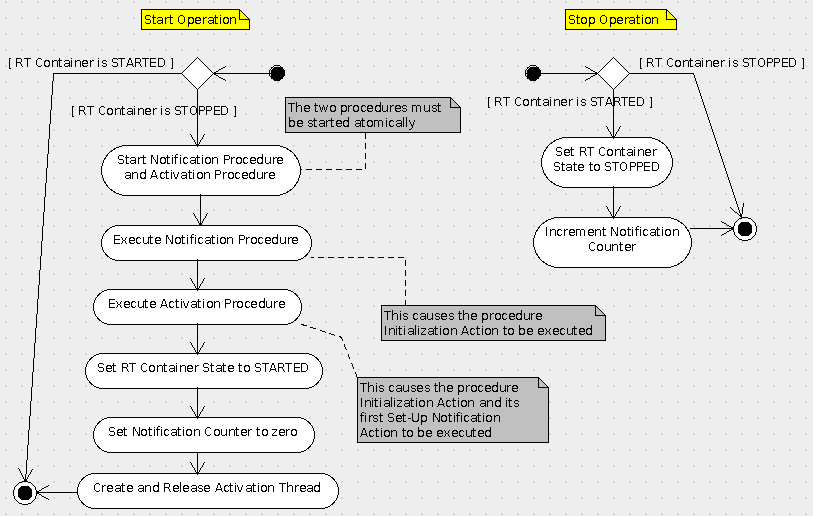
\includegraphics[scale=0.39,keepaspectratio=true]{RTStartStop.png}
 \caption{Start and Stop Operations for RT Containers}
 \label{fig:RTStartStop}
\end{figure}

When a RT Container is stopped, the behaviour shown in the activity diagram in the right-hand side of figure \ref{fig:RTStartStop} is executed. The Stop operation only has an effect if the container is in state STARTED when the operation causes the container to be placed in state STOPPED and the Notification Counter to be incremented. The latter results in one last notification being sent to the Activation Thread. This notification is necessary to ensure an orderly termination of the thread and of the Activation and Notification Procedures. 

When a RT Container is notified, the following behaviour is executed:

\begin{enumerate} 
\item If the RT Container is in state STOPPED, then no further action is performed;
\item If the RT Container is in state STARTED, then its Notification Procedure is executed.
\end{enumerate}

The behaviour of the \emph{Activation Thread} is expressed by the following pseudo-code:

\lstset{language=C,caption={Pseudo-code of Activation Thread},label=code:pseudoCodeActivationThread}
\begin{lstlisting}
while true do {
  wait until Notification Counter is greater than 0;
  decrement Notification Counter;
  execute Activation Procedure;
  
  if (Activation Procedure has terminated) then {
    put RT Container in STOPPED state;
    execute Notification Procedure;
    break;
  }

  if (RT Container is in state STOPPED) then {
    execute Activation Procedure;
    execute Notification Procedure;
    break;
  }
}
\end{lstlisting}

The thread executes a loop which starts with a check on whether there are any pending notifications (the Notification Counter holds the number of pending notifications). If there is a pending notification (i.e. if the Notification Counter is greater than zero), the thread decrements the Notification Counter and then executes the Activation Procedure (which causes the container's functional behaviour to be executed). The thread terminates when the Activation Procedure has terminated or when the RT container has been stopped. In the former case (Activation Procedure has autonomously terminated), the RT Container is put in the STOPPED state and the Notification Procedure is executed one last time before the thread exits; in the latter case (RT Container has been stopped), both procedures are executed one last time. This last execution is intended to give the procedures a chance to perform their finalization behaviour.

\begin{figure}[ht]
 \centering
 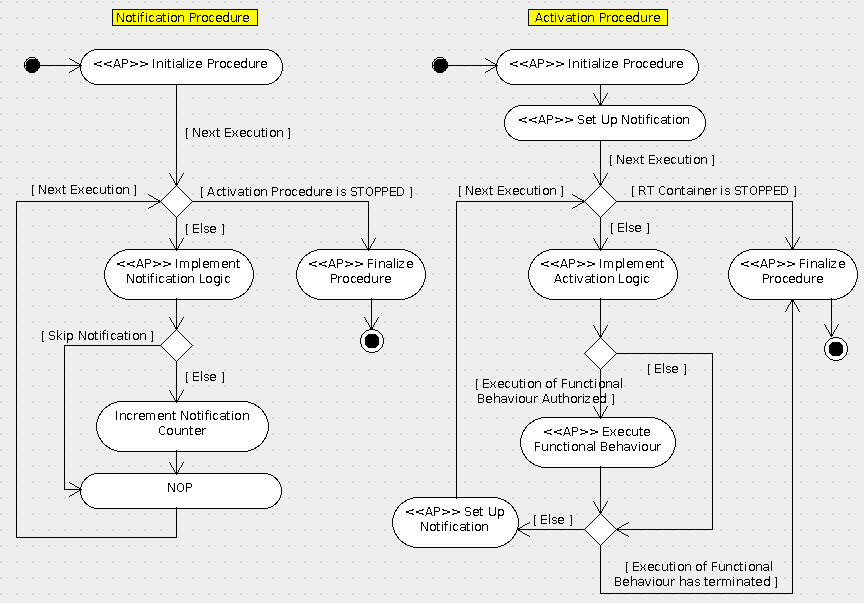
\includegraphics[scale=0.39,keepaspectratio=true]{RTContainer.png}
 % PRD.png: 474x227 pixel, 72dpi, 16.72x8.01 cm, bb=0 0 474 227
 \caption{RT Container Procedures}
 \label{fig:RTContainerProcedures}
\end{figure}

The behaviour of the \emph{Activation Procedure} and of the \emph{Notification Procedure} is shown in the
activity diagrams in Figure \ref{fig:RTContainerProcedures}. The definition of the two procedures makes use of the
“adaptation point” stereotype to identify the parts of the container behaviour which are
application-specific. Applications are therefore expected to extend the two procedures by inserting
their own application-specific behaviour (by contrast, the behaviour of the Activation Thread is invariant and is fully defined at FW Profile level).

When the Activation Procedure is executed for the first time (i.e. after the Activation Thread
has been started), it initializes itself and sets up the first notification of the Activation Thread.
The form of the notification is application-specific. Typically, the setting up of a notification
may consist of one of the following:

\begin{enumerate} 
\item A request that the Activation Thread be notified at some time in the future;
\item A call-back registration to request to be notified when a certain software condition
arises (e.g. a variable changes value, a message arrives, etc);
\item A request to be notified when a hardware interrupt is asserted.
\end{enumerate}

Note that the notification may only need to be set up once when the Activation Procedure is initialized or it may need to be set up at every execution cycle. Note also that the same RT Container may set up different notification requests in the same execution cycle or it may set up notification requests of different kinds at different execution cycles. For this reason, the "Set-Up Notification" in the Activation Procedure is placed both at the beginning of the procedure (to be executed once at initialization time) and inside the loop (to be executed after each execution of the functional behaviour).

When a notification arrives (i.e. when the user of the container executes the Notification Procedure and this increments the Notification Counter), the Activation Thread is woken up and it executes the Activation Procedure. The procedure checks whether the RT Container has been stopped. If this is the case, the procedure performs its finalization action and then terminates. Otherwise, the procedure checks whether the functional behaviour should be executed (this is done by the "Implement Activation Logic" action) and, if so, it executes it. Afterwards, the procedure sets up the next notification (if one is needed) and then checks whether the execution of the functional behaviour has been completed. If this is so, the procedure terminates. Otherwise it waits for the next notification.

The procedure initialization and finalization actions are adaptation points which are defined at application level. Similarly, the action to set up the notification for the Activation Thread and to implement the activation logic must also be defined at application level. The latter could, for instance, be used to implement a filter which decides which notifications to process and which ones to ignore.

The Notification Procedure acts as an intermediary
between the source of the notification event and the notification trigger to the Activation
Thread. Such an intermediary may be useful to: (a) filter notification events, or (b) buffer
notification requests so as to allow the Activation Procedure to handle bursts of notifications.
With reference to the activity diagram in Figure \ref{fig:RTContainerProcedures}, the filtering 
and buffering of notification requests is done in the (application-specific) action “Implement Notification Logic”.

As already noted, the Notification Procedure runs on a thread that is external to the RT
Container: the Notification Procedure is executed by an external thread when the notification
event has occurred. Thus, the logic leading to the notification of the Activation Thread is as
follows:

\begin{fw_enumerate}
\item The Activation Procedure makes a request to be notified when a certain event occurs
(this could, for instance, be done by registering with an external component to be
notified when a certain condition occurs);
\item When the event occurs, the Notification Procedure is executed by the source of the
event;
\item The Notification Procedure evaluates the event and may decide to notify the
Activation Thread;
\item The Notification Procedure notifies the Activation Thread by incrementing the Notification Counter;
\item In response to the notification, the Activation Thread executes the Activation Procedure which may execute the
functional behaviour encapsulated by the RT Container;
\item The Activation Procedure sets up the next notification request.

\end{fw_enumerate}

This cycle is broken when either the Activation Procedure decides that the execution of the
functional behaviour has been completed or when the RT Container is stopped. Either of these
events results in the RT Container and its two procedures terminating.

The Notification Procedure may be executed both by the Activation Thread and by an external thread. For this reason, in many cases, it will be necessary to ensure that it is executed in mutual exclusion.

Note finally that, in this section, the term "event" encompasses both asynchronous occurrences (such as the arrival of hardware interrupts from an external source) or synchronous occurrences (such as periodic signals generated by an operating system). 